\chapter{Teoria}

\section{Stack TCP/IP}
Per effettuare comunicazioni tramite internet, vi è il bisogno che tutti i dispositivi connessi rispettino determinati meccanismi; questo si rende necessario a causa dell'elevata eterogeneità derivata da hardware e software differenti.
Questi meccanismi, che prendono il nome di \textit{protocolli}, sono strutturati secondo diversi layer (livelli) formando lo stack TCP/IP.  \\
Sebbene l'idea originale prevedesse un modello composto da sette livelli, de facto lo schema attualmente in uso ne prevede solamente quattro. Nonostante ciò, nella terminologia informatica la numerazione è rimasta quella precedente.

\begin{table}[htb]
	\centering
	\begin{tabular}{| l | c |}
		\hline
		Livello 7 & Applicativo
		\\
		\hline
		Livello 4 & Trasporto
		\\
		\hline
		Livello 3 & Rete
		\\
		\hline
		Livello 2 & Fisico
		\\
		\hline
		
	\end{tabular}
	\caption{Livelli dello stack TCP/IP}
	\label{tab:stack}
\end{table}

\subsection{Funzionamento dello stack TCP/IP}
%Si consideri l'esempio dell'invio di una lettera tramite il servizio di poste. La procedura da seguire è la seguente:
%
%\begin{enumerate}
%	\item Il mittente scrive il contenuto del messaggio su un foglio e successivamente lo inserisce nella busta.
%	\item Il mittente scrive, nella busta, il nominativo del destinatario.
%	\item Il mittente scrive il CAP e l'indirizzo del ricevente.
%	\item Il mittente, dopo aver incollato il francobollo, consegna la busta al servizio di poste.
%\end{enumerate}
%
%Si noti che la sequenza di eventi che si verifica per la ricezione della lettera riflette le operazioni effettuate per l'invio, ma in ordine inverso:
%\begin{enumerate}
%	\item Viene controllata la presenza del francobollo.
%	\item Il postino legge l'indirizzo del destinatario e consegna la lettera.
%	\item Verrà letto il nominativo per individuare a quale inquilino è diretta.
%	\item Il destinatario apre la busta e legge il contenuto del messaggio.
%\end{enumerate}
%
%La sequenza di eventi descritta rappresenta ciò che avviene quando si comunica tramite internet. Ad ogni livello dello stack, infatti, vi è un protocollo che aggiunge una sua intestazione (\textit{header}) al pacchetto del mittente, ad iniziare dal livello più alto disponibile per quel dispositivo e il ricevente le valuterà in ordine inverso. Ad ogni layer il protocollo utilizzato può essere differente; fondamentale, ovviamente, che questo sia supportato da entrambi gli attori della conversazione.\\
%La procedura dell'inserimento degli header prende il nome di \textit{incapsulamento}.
%\\
Il meccanismo dello stack prevede che ad ogni livello vengano aggiunti al messaggio delle intestazioni (header), che verranno valutate dal ricevente nell'ordine inverso rispetto a quello del mittente.
Questa procedura prende il nome di \textit{incapsulamento} ed è riassunta nella seguente figura:


\begin{figure}[h]
	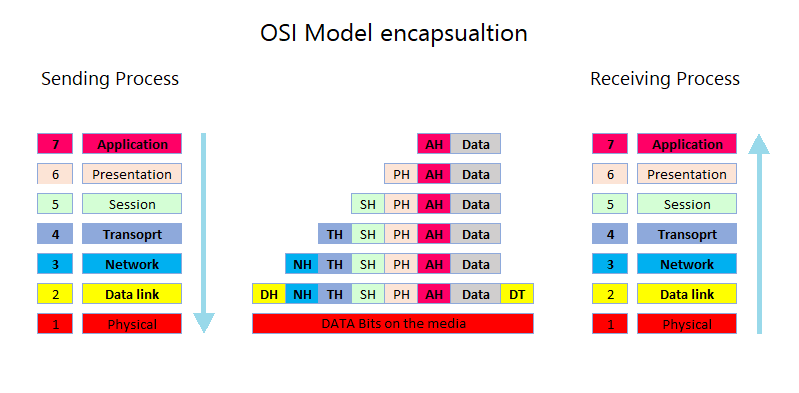
\includegraphics[width=\textwidth]{figures/incapsulamento.png}
	\caption{METTERE RIFERIMENTO IMMAGINE: http://infodoc.altervista.org/sistemi-e-reti/incapsulamento/}
	\label{incapsulamento}
\end{figure}

\subsection{Header per il fingerprinting}
Gli header aggiunti ad ogni livello sono formati da vari campi contententi informazioni utili per la comunicazione, e il valore che questi assumono in determinate situazioni è dipendente dal sistema operativo che si sta utilizzando.

Si prenda ad esempio l'header del protocollo TCP:\\

\begin{figure}[H]
	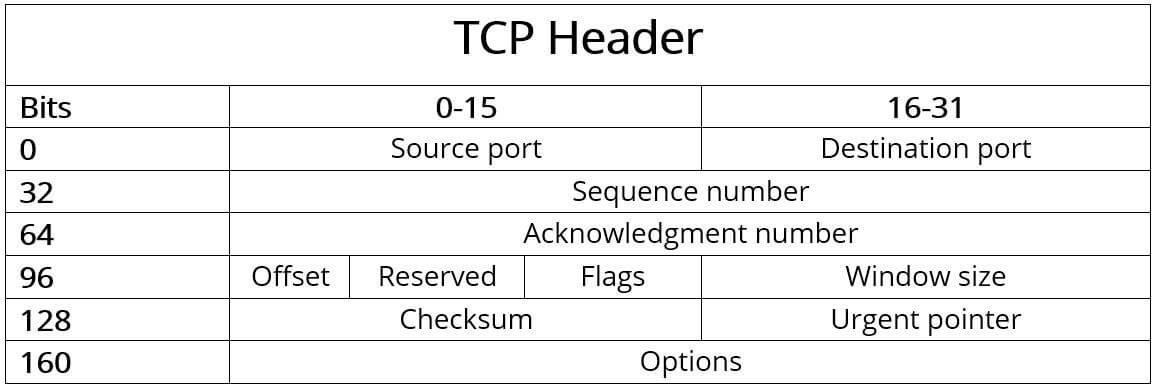
\includegraphics[width=\textwidth]{figures/headerTCP.JPG}
	\caption{METTERE RIFERIMENTO IMMAGINE: https://www.ionos.it/digitalguide/server/know-how/presentazione-tcp/}
	\label{headerTCP}
\end{figure}

Il campo \textit{option} permette di segnalare al ricevente l'uso di alcune opzioni di comunicazione, come il window scaling; il loro supporto e l'effettivo utilizzo, essendo queste facoltative e quindi peculiari di specifici sistemi operativi, rivestono quindi particolare importanza ai fini del fingerprinting.
Esempi analoghi si possono trovare nei protocolli di tutti i livelli dello stack, e l'unione delle informazioni acquisite consente di poter individuare con una discreta precisione il sistema operativo del dispositivo target.